\texttt{}~\\
\textbf{Resources}\\
Besides downloading all TimeTree species data
(\texttt{Eukaryota\_species.nwk}) we also need to manually query the
website for the 476 STRING eukaryotes
(\texttt{476\_ncbi\_eukaryotes.txt}). The file is called
\texttt{476\_ncbi\_eukaryotes.txt} because it contains updated NCBI
Taxonomy names rather than STRING outdated names. This ensures better
results.

\begin{Shaded}
\begin{Highlighting}[]
\KeywordTok{download_if_missing}\NormalTok{(}
  \KeywordTok{paste0}\NormalTok{(}\StringTok{"http://timetree.org/ajax/direct_download"}\NormalTok{,}
         \StringTok{"?direct-download-format=newick"}\NormalTok{,}
         \StringTok{"&direct-download-id=23070"}\NormalTok{,}
         \StringTok{"&direct-download-rank=species"}\NormalTok{),}
  \StringTok{"Eukaryota_species.nwk"}
\NormalTok{)}
\end{Highlighting}
\end{Shaded}

\texttt{timetree\_newick} is the tree obtained by manually uploading
\texttt{476\_ncbi\_eukaryotes.txt} to the TimeTree website.
\texttt{tree\_85k} is the complete Eukaryota tree we have just
downloaded.

\begin{Shaded}
\begin{Highlighting}[]
\CommentTok{# loading species names and taxon ids}
\KeywordTok{load}\NormalTok{(}\StringTok{"../data/string_eukaryotes.rda"}\NormalTok{)}

\CommentTok{# loading newick tree manually obtained from timetree}
\NormalTok{timetree_newick <-}\StringTok{ }\KeywordTok{read.tree}\NormalTok{(}\StringTok{"download/timetree_335_eukaryotes.nwk"}\NormalTok{)}

\CommentTok{# the following genera names are unreliable and should not be searched for}
\NormalTok{duplicated_genera <-}\StringTok{ }\KeywordTok{scan}\NormalTok{(}\StringTok{"duplicated_genera.txt"}\NormalTok{, }\DataTypeTok{what =} \StringTok{"character"}\NormalTok{)}

\CommentTok{# loading all TimeTree species data we have just download (85000 species)}
\NormalTok{tree_85k <-}\StringTok{ }\KeywordTok{read.tree}\NormalTok{(}\StringTok{"download/Eukaryota_species.nwk"}\NormalTok{)}
\end{Highlighting}
\end{Shaded}

\textbf{Unfound species with matching genera}\\
Some of the 476 STRING eukaryotes are not present in the TimeTree
database. However, sometimes TimeTree does contain tree data for closely
related species (e.g.~\emph{Monosiga brevicollis} is not present, but
\emph{Monosiga ovata} is). Therefore, we can use these closely related
species as proxies for the actual species. This is done by searching for
genera names in the complete database (\texttt{Eukaryota\_species.nwk}).
In the given \emph{Monosiga brevicollis} example, we search for
\emph{Monosiga} in the complete database. We see that there is
information for at least one other species of the \emph{Monosiga} genus
(in this case, \emph{Monosiga ovata}), so we add \emph{Monosiga
brevicollis} as a sister branch to the found species.

When you search for a term in TimeTree, it uses a synonym list obtained
from NCBI to try to resolve it. Sometimes TimeTree will resolve a
searched term to a scientific name different from the one you searched
for. The problem with this is that TimeTree does not make it obvious
that it is returning a different term. The first step is to find out
which species resolved to different names in the
\texttt{timetree\_335\_eukaryotes.nwk} file:

\begin{Shaded}
\begin{Highlighting}[]
\CommentTok{# plot(timetree_newick %>% ladderize, type = "cladogram", use.edge.length = F)}

\CommentTok{# replacing timetree species underscores with spaces}
\NormalTok{timetree_newick[[}\StringTok{"tip.label"}\NormalTok{]] }\OperatorTok\StringTok{ }\KeywordTok{str_replace_all}\NormalTok{(}\StringTok{"_"}\NormalTok{, }\StringTok{" "}\NormalTok{)}

\CommentTok{# which timetree species' names exactly match with ncbi's}
\NormalTok{taxid_indexes <-}\StringTok{ }\NormalTok{timetree_newick[[}\StringTok{"tip.label"}\NormalTok{]] }\OperatorTok\StringTok{ }\KeywordTok{match}\NormalTok{(string_eukaryotes[[}\StringTok{"ncbi_name"}\NormalTok{]])}

\CommentTok{# find out which timetree species names didn't exactly match ncbi's}
\NormalTok{unmatched_names <-}\StringTok{ }\NormalTok{timetree_newick[[}\StringTok{"tip.label"}\NormalTok{]] }\OperatorTok\StringTok{ }\NormalTok{magrittr}\OperatorTok{::}\KeywordTok{extract}\NormalTok{(taxid_indexes }\OperatorTok\StringTok{ }\NormalTok{is.na)}
\KeywordTok{print}\NormalTok{(unmatched_names)}
\end{Highlighting}
\end{Shaded}

\begin{verbatim}
## [1] "Cercospora fijiensis"     "Arthroderma benhamiae"   
## [3] "Macropus eugenii"         "Ostreococcus lucimarinus"
## [5] "Oryza nivara"
\end{verbatim}

\begin{Shaded}
\begin{Highlighting}[]
\CommentTok{# manually creating lookup table to be joined}
\NormalTok{ncbi_to_timetree <-}\StringTok{ }\KeywordTok{tribble}\NormalTok{(}
  \OperatorTok{~}\NormalTok{timetree_name,              }\OperatorTok{~}\NormalTok{ncbi_name,}
  \StringTok{"Cercospora fijiensis"}\NormalTok{,      }\StringTok{"Pseudocercospora fijiensis"}\NormalTok{,}
  \StringTok{"Arthroderma benhamiae"}\NormalTok{,     }\StringTok{"Trichophyton benhamiae"}\NormalTok{,}
  \StringTok{"Macropus eugenii"}\NormalTok{,          }\StringTok{"Notamacropus eugenii"}\NormalTok{,}
  \StringTok{"Ostreococcus lucimarinus"}\NormalTok{,  }\StringTok{"Ostreococcus sp. 'lucimarinus'"}\NormalTok{,}
  \StringTok{"Oryza nivara"}\NormalTok{,              }\StringTok{"Oryza sativa f. spontanea"}
\NormalTok{)}

\CommentTok{# joining info}
\NormalTok{species_dictionary <-}\StringTok{ }\NormalTok{string_eukaryotes }\OperatorTok\StringTok{ }\KeywordTok{left_join}\NormalTok{(ncbi_to_timetree)}

\CommentTok{# coalescing NAs to ncbi_name}
\NormalTok{species_dictionary }\OperatorTok
\StringTok{  }\KeywordTok{mutate}\NormalTok{(}\DataTypeTok{timetree_name =} \KeywordTok{coalesce}\NormalTok{(timetree_name, ncbi_name)) }\OperatorTok
\StringTok{  }\KeywordTok{mutate}\NormalTok{(}\DataTypeTok{timetree_name =} \KeywordTok{ifelse}\NormalTok{(timetree_name }\OperatorTok\StringTok{ }\NormalTok{timetree_newick[[}\StringTok{"tip.label"}\NormalTok{]], timetree_name, }\OtherTok{NA}\NormalTok{))}
\end{Highlighting}
\end{Shaded}

Now we can start looking for unfound species genera in the complete tree
data.

\begin{Shaded}
\begin{Highlighting}[]
\CommentTok{# annotating genera}
\NormalTok{species_dictionary }\OperatorTok
\StringTok{  }\KeywordTok{mutate}\NormalTok{(}\DataTypeTok{genus_search =} \KeywordTok{coalesce}\NormalTok{(timetree_name, ncbi_name) }\OperatorTok
\StringTok{  }\KeywordTok{strsplit}\NormalTok{(}\StringTok{" "}\NormalTok{) }\OperatorTok
\StringTok{  }\KeywordTok{sapply}\NormalTok{(}\StringTok{"["}\NormalTok{, }\DecValTok{1}\NormalTok{))}

\CommentTok{# unique genera}
\NormalTok{selected_genera <-}\StringTok{ }\NormalTok{species_dictionary[[}\StringTok{"genus_search"}\NormalTok{]] }\OperatorTok\StringTok{ }\NormalTok{unique}

\CommentTok{# these are unreliable selected_genera:}
\NormalTok{unreliable_genera <-}\StringTok{ }\KeywordTok{intersect}\NormalTok{(selected_genera, duplicated_genera)}

\CommentTok{# ensuring a cleaner newick file with only necessary data}
\CommentTok{# this is actually really important}
\NormalTok{tree_85k[[}\StringTok{"node.label"}\NormalTok{]] <-}\StringTok{ }\OtherTok{NULL}
\NormalTok{tree_85k[[}\StringTok{"edge.length"}\NormalTok{]] <-}\StringTok{ }\OtherTok{NULL}

\CommentTok{# replacing timetree's underscores with spaces}
\NormalTok{tree_85k[[}\StringTok{"tip.label"}\NormalTok{]] }\OperatorTok\StringTok{ }\KeywordTok{str_replace_all}\NormalTok{(}\StringTok{"_"}\NormalTok{, }\StringTok{" "}\NormalTok{)}

\CommentTok{# storing genus}
\NormalTok{tree_85k[[}\StringTok{"tip.genus"}\NormalTok{]] <-}\StringTok{ }\KeywordTok{sapply}\NormalTok{(}\KeywordTok{strsplit}\NormalTok{(tree_85k[[}\StringTok{"tip.label"}\NormalTok{]],}\StringTok{" "}\NormalTok{), }\StringTok{"["}\NormalTok{, }\DecValTok{1}\NormalTok{)}
\NormalTok{tree_85k_genera <-}\StringTok{ }\NormalTok{tree_85k[[}\StringTok{"tip.genus"}\NormalTok{]] }\OperatorTok\StringTok{ }\NormalTok{unique}

\CommentTok{# subtracting unreliable genera}
\NormalTok{tree_85k_genera }\OperatorTok\StringTok{ }\KeywordTok{setdiff}\NormalTok{(unreliable_genera)}

\CommentTok{# keeping only selected genera, including unreliable ones}
\NormalTok{tree_genus <-}\StringTok{ }\NormalTok{tree_85k }\OperatorTok\StringTok{ }\KeywordTok{keep.tip}\NormalTok{(., tip.label[tip.genus }\OperatorTok\StringTok{ }\NormalTok{selected_genera])}
\NormalTok{tree_genus[[}\StringTok{"tip.genus"}\NormalTok{]] <-}\StringTok{ }\KeywordTok{sapply}\NormalTok{(}\KeywordTok{strsplit}\NormalTok{(tree_genus[[}\StringTok{"tip.label"}\NormalTok{]],}\StringTok{" "}\NormalTok{), }\StringTok{"["}\NormalTok{, }\DecValTok{1}\NormalTok{)}

\CommentTok{# unfound species which genera are present in the 85k tree}
\NormalTok{unfound_species <-}\StringTok{ }\NormalTok{species_dictionary }\OperatorTok
\StringTok{  }\KeywordTok{filter}\NormalTok{(}\KeywordTok{is.na}\NormalTok{(timetree_name) }\OperatorTok{&}\StringTok{ }\NormalTok{genus_search }\OperatorTok\StringTok{ }\NormalTok{tree_85k_genera)}
\end{Highlighting}
\end{Shaded}

Once we figured out which species have proxy genera in the complete
data, we can start filling them in as sister branches.

\begin{Shaded}
\begin{Highlighting}[]
\CommentTok{# for each unfound species which genus is present in the 85k tree,}
\ControlFlowTok{for}\NormalTok{(i }\ControlFlowTok{in} \DecValTok{1}\OperatorTok{:}\KeywordTok{nrow}\NormalTok{(unfound_species))\{}
  \CommentTok{# we search for all species of this genus ("sister species") in the 85k tree}
  \CommentTok{# this part is tricky because bind.tip rebuilds the tree from scratch}
  \CommentTok{# so we need to keep removing underscores. there are better ways to do this.}
\NormalTok{  tip_genus <-}\StringTok{ }\NormalTok{tree_genus[[}\StringTok{"tip.label"}\NormalTok{]] }\OperatorTok\StringTok{ }\KeywordTok{strsplit}\NormalTok{(}\StringTok{"[_ ]"}\NormalTok{) }\OperatorTok\StringTok{ }\KeywordTok{sapply}\NormalTok{(}\StringTok{"["}\NormalTok{, }\DecValTok{1}\NormalTok{)}
\NormalTok{  sister_species <-}\StringTok{ }\NormalTok{tree_genus[[}\StringTok{"tip.label"}\NormalTok{]][tip_genus }\OperatorTok{==}\StringTok{ }\NormalTok{unfound_species[[i, }\StringTok{"genus_search"}\NormalTok{]]]}
  \CommentTok{# we obtain the sister_species' most recent common ancestor (MRCA)}
  \CommentTok{# c(.[1]) is a hack because the MRCA function only works with at least 2 nodes}
\NormalTok{  where <-}\StringTok{ }\KeywordTok{getMRCA}\NormalTok{(tree_genus, sister_species }\OperatorTok\StringTok{ }\KeywordTok{c}\NormalTok{(.[}\DecValTok{1}\NormalTok{]))}
  \CommentTok{# and then add a leaf node linked to this MRCA}
\NormalTok{  tree_genus }\OperatorTok\StringTok{ }\KeywordTok{bind.tip}\NormalTok{(}\DataTypeTok{tip.label =}\NormalTok{ unfound_species[[i, }\StringTok{"ncbi_name"}\NormalTok{]], }\DataTypeTok{where =}\NormalTok{ where)}
\NormalTok{\}}

\CommentTok{# for some reason bind.tip adds underscores to species names}
\NormalTok{tree_genus[[}\StringTok{"tip.label"}\NormalTok{]] }\OperatorTok\StringTok{ }\KeywordTok{str_replace_all}\NormalTok{(}\StringTok{"_"}\NormalTok{, }\StringTok{" "}\NormalTok{)}

\CommentTok{# keeping track of found species}
\NormalTok{found_species <-}\StringTok{ }\NormalTok{species_dictionary }\OperatorTok\StringTok{ }\KeywordTok{filter}\NormalTok{(}\OperatorTok{!}\KeywordTok{is.na}\NormalTok{(timetree_name) }\OperatorTok{|}\StringTok{ }\NormalTok{genus_search }\OperatorTok\StringTok{ }\NormalTok{tree_85k_genera)}
\CommentTok{# forced_name means it either was found in timetree or we forced it by looking at genera names}
\NormalTok{found_species }\OperatorTok\StringTok{ }\KeywordTok{mutate}\NormalTok{(}\DataTypeTok{forced_name =} \KeywordTok{coalesce}\NormalTok{(timetree_name, ncbi_name))}

\CommentTok{# so we keep only found species in this tree we are building (timetree + forced by genera)}
\NormalTok{tree_genus }\OperatorTok\StringTok{ }\KeywordTok{keep.tip}\NormalTok{(found_species[[}\StringTok{"forced_name"}\NormalTok{]])}

\CommentTok{# which found_species rows correspond to each tip.label?}
\NormalTok{match_tiplabel_name <-}\StringTok{ }\KeywordTok{match}\NormalTok{(tree_genus[[}\StringTok{"tip.label"}\NormalTok{]], found_species[[}\StringTok{"forced_name"}\NormalTok{]])}

\NormalTok{tree_genus }\OperatorTok\StringTok{ }\KeywordTok{list_modify}\NormalTok{(}
\CommentTok{# converting to ncbi taxids}
  \DataTypeTok{tip.label =}\NormalTok{ found_species[[}\StringTok{"new_taxid"}\NormalTok{]][match_tiplabel_name]}
\NormalTok{)}
\end{Highlighting}
\end{Shaded}

\textbf{Species of unfound genera}\\
In this part, we try to fill in the remaining missing species (those
which genera were not found in TimeTree) by searching for their closest
relatives (according to NCBI Taxonomy) that are present in the current
tree. Once we find its two closest relatives, we can add the missing
species as a branch from their LCA. This is a conservative approach.

\begin{Shaded}
\begin{Highlighting}[]
\CommentTok{# converting ncbi phylo to igraph}
\NormalTok{graph_ncbi <-}\StringTok{ }\KeywordTok{read.tree}\NormalTok{(}\StringTok{"tree_ncbi.nwk"}\NormalTok{) }\OperatorTok\StringTok{ }\KeywordTok{as.igraph.phylo}\NormalTok{(}\DataTypeTok{directed =} \OtherTok{TRUE}\NormalTok{)}

\CommentTok{# converting phylo to igraph}
\NormalTok{graph_genus <-}\StringTok{ }\KeywordTok{as.igraph.phylo}\NormalTok{(tree_genus, }\DataTypeTok{directed =} \OtherTok{TRUE}\NormalTok{)}

\CommentTok{# for each species which genus is not in timetree}
\CommentTok{# we'll look for its two closest species (in the NCBI tree) which are present in the tree_genus we just built}
\NormalTok{unfound_genera <-}\StringTok{ }\NormalTok{species_dictionary }\OperatorTok\StringTok{ }\KeywordTok{filter}\NormalTok{(}\KeywordTok{is.na}\NormalTok{(timetree_name) }\OperatorTok{&}\StringTok{ }\OperatorTok{!}\NormalTok{genus_search }\OperatorTok\StringTok{ }\NormalTok{tree_85k_genera)}

\CommentTok{# this is the igraph equivalent of "phylo_tree$tip.label"}
\NormalTok{tip_nodes <-}\StringTok{ }\KeywordTok{V}\NormalTok{(graph_ncbi)[}\KeywordTok{degree}\NormalTok{(graph_ncbi, }\DataTypeTok{mode =} \StringTok{"out"}\NormalTok{) }\OperatorTok{==}\StringTok{ }\DecValTok{0}\NormalTok{]}

\CommentTok{# undirected distances between all species nodes}
\NormalTok{tip_distances <-}\StringTok{ }\NormalTok{graph_ncbi }\OperatorTok
\StringTok{  }\KeywordTok{distances}\NormalTok{(}\DataTypeTok{v =}\NormalTok{ tip_nodes, }\DataTypeTok{to =}\NormalTok{ tip_nodes, }\DataTypeTok{mode =} \StringTok{"all"}\NormalTok{) }\OperatorTok
\StringTok{  }\KeywordTok{as_tibble}\NormalTok{(}\DataTypeTok{rownames =} \StringTok{"from"}\NormalTok{) }\OperatorTok
\StringTok{  }\KeywordTok{pivot_longer}\NormalTok{(}\OperatorTok{-}\NormalTok{from, }\DataTypeTok{names_to =} \StringTok{"to"}\NormalTok{, }\DataTypeTok{values_to =} \StringTok{"distance"}\NormalTok{)}

\CommentTok{# removing self references (zero distances)}
\NormalTok{tip_distances }\OperatorTok\StringTok{ }\KeywordTok{filter}\NormalTok{(distance }\OperatorTok{>}\StringTok{ }\DecValTok{0}\NormalTok{)}

\CommentTok{# we only want to search for species of unfound genera}
\NormalTok{tip_distances }\OperatorTok\StringTok{ }\KeywordTok{inner_join}\NormalTok{(unfound_genera }\OperatorTok\StringTok{ }\KeywordTok{select}\NormalTok{(}\DataTypeTok{from =}\NormalTok{ new_taxid))}

\CommentTok{# we only want to find species already present in the genus_tree}
\NormalTok{tip_distances }\OperatorTok\StringTok{ }\KeywordTok{inner_join}\NormalTok{(found_species }\OperatorTok\StringTok{ }\KeywordTok{select}\NormalTok{(}\DataTypeTok{to =}\NormalTok{ new_taxid))}

\CommentTok{# we only want the two closest relatives}
\NormalTok{tip_distances }\OperatorTok
\StringTok{  }\KeywordTok{group_by}\NormalTok{(from) }\OperatorTok
\StringTok{  }\KeywordTok{top_n}\NormalTok{(}\OperatorTok{-}\DecValTok{2}\NormalTok{, distance) }\OperatorTok\StringTok{ }\CommentTok{# top 2 smallest distances}
\StringTok{  }\KeywordTok{top_n}\NormalTok{(}\DecValTok{2}\NormalTok{, to) }\CommentTok{# more than 2 species have the same smallest distance, so we get the first ones}

\CommentTok{# out distance matrix between all nodes in tree, needed to find MRCAs}
\NormalTok{out_distances <-}\StringTok{ }\NormalTok{graph_genus }\OperatorTok\StringTok{ }\KeywordTok{distances}\NormalTok{(}\DataTypeTok{mode =} \StringTok{"out"}\NormalTok{)}

\CommentTok{# for each species of unfound genera,}
\CommentTok{# we find the MRCA for its two closest relatives}
\NormalTok{unfound_genera_mrca <-}\StringTok{ }\NormalTok{tip_distances }\OperatorTok\StringTok{ }\KeywordTok{group_by}\NormalTok{(from) }\OperatorTok\StringTok{ }\KeywordTok{summarise}\NormalTok{(}\DataTypeTok{mrca =}\NormalTok{ \{}
  \CommentTok{# which rows have no infinite distances? the last one represents the MRCA}
\NormalTok{  mrca_row_index <-}\StringTok{ }\KeywordTok{max}\NormalTok{(}\KeywordTok{which}\NormalTok{(}\KeywordTok{rowSums}\NormalTok{(}\KeywordTok{is.infinite}\NormalTok{(out_distances[, to])) }\OperatorTok{==}\StringTok{ }\DecValTok{0}\NormalTok{))}
  \KeywordTok{rownames}\NormalTok{(out_distances)[mrca_row_index]}
\NormalTok{\})}

\CommentTok{# adding unfound genera species nodes}
\NormalTok{graph_genus }\OperatorTok\StringTok{ }\KeywordTok{add_vertices}\NormalTok{(}\KeywordTok{nrow}\NormalTok{(unfound_genera_mrca), }\DataTypeTok{color =} \StringTok{"red"}\NormalTok{, }\DataTypeTok{attr =} \KeywordTok{list}\NormalTok{(}\DataTypeTok{name =}\NormalTok{ unfound_genera_mrca[[}\StringTok{"from"}\NormalTok{]]))}

\CommentTok{# defining unfound genera species edges}
\CommentTok{# edges_to_add[1] -> edges_to_add[2], edges_to_add[2] -> edges_to_add[3]...}
\NormalTok{edges_to_add <-}\StringTok{ }\KeywordTok{V}\NormalTok{(graph_genus)[unfound_genera_mrca }\OperatorTok\StringTok{ }\KeywordTok{select}\NormalTok{(mrca, from) }\OperatorTok\StringTok{ }\NormalTok{t }\OperatorTok\StringTok{ }\NormalTok{as.vector]}\OperatorTok{$}\NormalTok{name}

\CommentTok{# connecting species leafs to the supposed MRCA}
\NormalTok{graph_genus }\OperatorTok\StringTok{ }\KeywordTok{add_edges}\NormalTok{(}\KeywordTok{V}\NormalTok{(graph_genus)[edges_to_add])}

\CommentTok{# plotting}
\CommentTok{# plot(as.undirected(graph_genus), layout = layout_as_tree(graph_genus), vertex.label = NA, vertex.size=2)}

\CommentTok{# finally converting to phylo format}
\NormalTok{phylo_graph_genus <-}\StringTok{ }\NormalTok{treeio}\OperatorTok{::}\KeywordTok{as.phylo}\NormalTok{(graph_genus)}

\CommentTok{# which species_dictionary rows correspond to each tip.label?}
\NormalTok{match_tiplabel_taxid <-}\StringTok{ }\KeywordTok{match}\NormalTok{(phylo_graph_genus[[}\StringTok{"tip.label"}\NormalTok{]], species_dictionary[[}\StringTok{"new_taxid"}\NormalTok{]])}

\NormalTok{phylo_graph_genus }\OperatorTok\StringTok{ }\KeywordTok{list_modify}\NormalTok{(}
  \CommentTok{# adding tip.alias (this is not exported with write.tree)}
  \DataTypeTok{tip.alias =}\NormalTok{ species_dictionary[[}\StringTok{"string_name"}\NormalTok{]][match_tiplabel_taxid],}
  \CommentTok{# converting back to string ids}
  \DataTypeTok{tip.label =}\NormalTok{ species_dictionary[[}\StringTok{"taxid"}\NormalTok{]][match_tiplabel_taxid]}
\NormalTok{)}

\CommentTok{# ensuring a cleaner newick file with only necessary data}
\NormalTok{phylo_graph_genus[[}\StringTok{"node.label"}\NormalTok{]] <-}\StringTok{ }\OtherTok{NULL}
\NormalTok{phylo_graph_genus[[}\StringTok{"edge.length"}\NormalTok{]] <-}\StringTok{ }\OtherTok{NULL}

\CommentTok{# usethis::use_data(phylo_graph_genus, overwrite = TRUE)}
\CommentTok{# write.tree(phylo_graph_genus, "../data/hybrid_tree.nwk")}
\end{Highlighting}
\end{Shaded}

\textbf{Ctenophora as sister to all animals}\\
According to TimeTree, Ctenophora remains as a sister group to Cnidaria.
We believe the most recent consensus in literature is to consider them a
sister group to all animals. The following code block moves
\emph{Mnemiopsis leidyi}, the only ctenophore in our analysis, to the
base of the metazoan lineage.

\begin{Shaded}
\begin{Highlighting}[]
\CommentTok{# reordering tip.labels}
\NormalTok{from_to <-}\StringTok{ }\KeywordTok{c}\NormalTok{(}
  \StringTok{"400682"}\NormalTok{ =}\StringTok{ "27923"}\NormalTok{,  }\CommentTok{# amphimedon to mnemiopsis}
  \StringTok{"10228"}\NormalTok{  =}\StringTok{ "400682"}\NormalTok{, }\CommentTok{# trichoplax to amphimedon}
  \StringTok{"27923"}\NormalTok{  =}\StringTok{ "10228"}   \CommentTok{# mnemiopsis to trichoplax}
\NormalTok{)}

\NormalTok{modified_phylo <-}\StringTok{ }\NormalTok{phylo_graph_genus}

\NormalTok{modified_phylo[[}\StringTok{"tip.label"}\NormalTok{]] }\OperatorTok\StringTok{ }\KeywordTok{recode}\NormalTok{(}\OperatorTok{!!!}\NormalTok{from_to)}

\KeywordTok{write.tree}\NormalTok{(modified_phylo, }\StringTok{"../data/hybrid_tree_modified.nwk"}\NormalTok{)}
\end{Highlighting}
\end{Shaded}

\begin{figure}
\centering
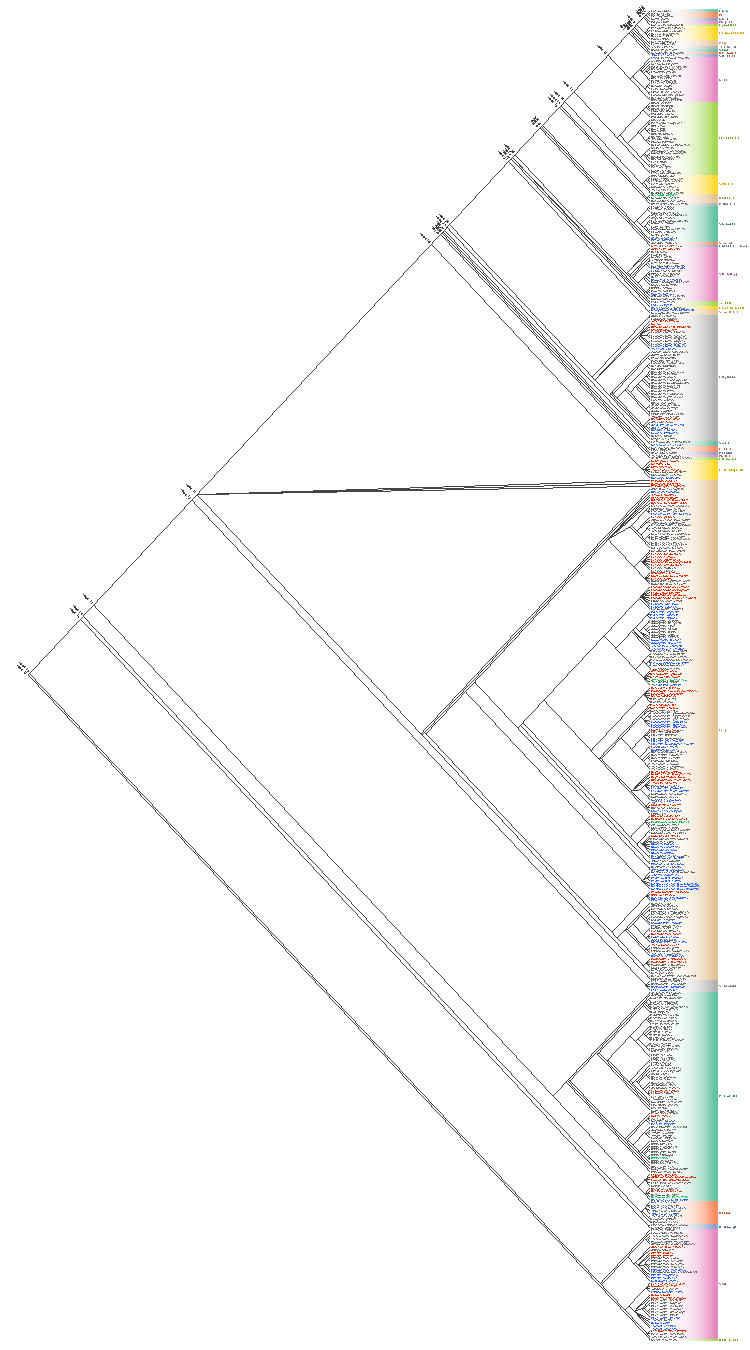
\includegraphics[width=\textwidth,height=0.95\textheight]{../data-raw/tree_hybrid.pdf}
\caption{Complete 476 eukaryotes tree. Green species have been filled in
by a genus proxy in TimeTree. Red species have been filled in by looking
at NCBI Taxonomy. Clade naming is described further in this document.}
\end{figure}
